\documentclass[12pt]{article}
\usepackage[spanish]{babel}
\usepackage{natbib}
\usepackage[hidelinks]{hyperref}
\usepackage[utf8x]{inputenc}
\usepackage{amsmath}
\usepackage{graphicx}
\graphicspath{{images/}}
\usepackage{parskip}
\usepackage{fancyhdr}
\usepackage{float}
\usepackage{array}
\usepackage{tabularx}
\usepackage{tikz}
\usetikzlibrary{positioning, arrows.meta}

\usepackage{vmargin}
\setmarginsrb{3 cm}{2.5 cm}{2.5 cm}{2.5 cm} {1 cm}{1.5 cm}{1 cm}{1.5 cm}

\title{Sistema Híbrido de Detección y Segmentación de Transporte Escolar en Tiempo Real}
\author{Kevin Andres Morocho Remache}
\date{\today}

\makeatletter
\let\thetitle\@title
\let\theauthor\@author
\let\thedate\@date
\makeatother

\pagestyle{fancy}
\fancyhf{}
\lhead{\thetitle}
\cfoot{\thepage}

\begin{document}

\renewcommand{\listtablename}{Lista de Tablas}
\renewcommand{\tablename}{Tabla}
\renewcommand{\listfigurename}{Lista de Figuras}
\renewcommand{\figurename}{Figura}

%%%%%%%%%%%%%%%%%%%%%%%%%%%%%%%%%%%%%%%%%%%%%%%%%%%%%%%%%%%%%%%%%%%%%%%%%%%%%%%%%%%%%%%%%
%%%%%%%%%%%%%  INICIO PORTADA  %%%%%%%%%%%%%%%%%%%%%%%%%%%%%%%%%%%%%%%%%%%%%%%%%%%%%%%%%%
%%%%%%%%%%%%%%%%%%%%%%%%%%%%%%%%%%%%%%%%%%%%%%%%%%%%%%%%%%%%%%%%%%%%%%%%%%%%%%%%%%%%%%%%%
\begin{titlepage}
	\centering
    % Nota: Coloca el archivo logo.png en la carpeta images/ para que se visualice en la compilación
    \includegraphics[width=0.5\linewidth]{logo.png}\\[1.0 cm]
    \textsc{\LARGE Universidad Politécnica Salesiana}\\[2.0 cm]
	\textsc{\Large VSC}\\[0.5 cm]
	\textsc{\large Visión por Computador}\\[0.5 cm]
	\rule{\linewidth}{0.2 mm} \\[0.4 cm]
	{ \huge \bfseries \thetitle}\\
	\rule{\linewidth}{0.2 mm} \\[1.5 cm]
	
 \begin{flushleft} \large
    \emph{Autor:}\\
	\theauthor 
 \end{flushleft}
 
  \begin{flushleft} \large
    \emph{Docente:}\\
	Ing. Vladímir Robles \\
  \end{flushleft}
  
  \vspace{0.8cm}
  {\large \href{https://github.com/KAndresMR/stereo_project_vision}{\textbf{[Ver Repositorio del Proyecto en GitHub]}} \\[0.4cm]
  \href{https://github.com/KAndresMR/stereo_project_vision/tree/refactor/optimize/parte2_detector/videos}{\textbf{[Ver Video de Demostración del Sistema]}}}
  
  \vfill

  {\large \thedate}

\end{titlepage}
%%%%%%%%%%%%%%%%%%%%%%%%%%%%%%%%%%%%%%%%%%%%%%%%%%%%%%%%%%%%%%%%%%%%%%%%%%%%%%%%%%%%%%%%%
%%%%%%%%%%%%%    FIN  PORTADA  %%%%%%%%%%%%%%%%%%%%%%%%%%%%%%%%%%%%%%%%%%%%%%%%%%%%%%%%%%
%%%%%%%%%%%%%%%%%%%%%%%%%%%%%%%%%%%%%%%%%%%%%%%%%%%%%%%%%%%%%%%%%%%%%%%%%%%%%%%%%%%%%%%%%

\tableofcontents
\listoftables
\listoffigures
\pagebreak

%%%%%%%%%%%%%%%%%%%%%%%%%%%%%%%%%%%%%%%%%%%%%%%%%%%%%%%%%%%%%%%%%%%%%%%%%%%%%%%%%%%%%%%%%
%%%%%%%%%%%%%    INICIO   TEXTO   %%%%%%%%%%%%%%%%%%%%%%%%%%%%%%%%%%%%%%%%%%%%%%%%%%%%%%%
%%%%%%%%%%%%%%%%%%%%%%%%%%%%%%%%%%%%%%%%%%%%%%%%%%%%%%%%%%%%%%%%%%%%%%%%%%%%%%%%%%%%%%%%%

\section{Introducción}
El desarrollo de sistemas de vigilancia inteligente vial y la asistencia automatizada al monitoreo de tráfico representan pilares fundamentales dentro de las aplicaciones modernas de la visión por computador \cite{bradski2000opencv}. En particular, la protección escolar en corredores viales urbanos exige mecanismos capaces de identificar de manera ininterrumpida, precisa y con baja latencia la presencia de vehículos de transporte infantil, con el propósito de prevenir accidentes en zonas de alta vulnerabilidad peatonal. 

Las aproximaciones contemporáneas suelen depender exclusivamente de redes neuronales convolucionales profundas y arquitecturas basadas en transformadores, las cuales ofrecen una precisión sobresaliente pero demandan una infraestructura de cómputo especializada con unidades de procesamiento gráfico (GPU) de alto rendimiento. En contraste, los entornos de monitoreo vial reales, especialmente en infraestructuras municipales descentralizadas o cámaras de seguridad comunitarias (CCTV), operan sobre hardware de recursos computacionales limitados (dispositivos de borde o computadores convencionales) \cite{dalal2005hog}. Asimismo, investigaciones recientes desarrolladas en el contexto universitario ecuatoriano han demostrado la viabilidad y el impacto de implementar sistemas inteligentes asistidos por visión artificial y aprendizaje por transferencia en escenarios locales de alta sensibilidad social y educativa \cite{robles2022inteligencia, robles2023mobile}.

El presente proyecto aborda este desafío mediante el diseño, optimización e implementación de una arquitectura de visión artificial híbrida y distribuida. En una primera capa de procesamiento en el borde (*Edge Computing*), se ejecuta un detector visual de alta velocidad implementado en el lenguaje C++ sobre la librería OpenCV, aprovechando descriptores geométricos clásicos basados en Histogramas de Gradientes Orientados (HOG) clasificados por una Máquina de Vectores de Soporte lineal (SVM) \cite{pedregosa2011scikit}. Una vez que este motor local detecta y valida la presencia persistente de un autobús escolar en el flujo de video en vivo, el sistema despliega mecanismos de concurrencia para capturar evidencias audiovisuales y transmitirlas de forma asíncrona hacia un servidor de backend en Python. En esta segunda etapa, una arquitectura de aprendizaje profundo YOLOv8 Nano (\emph{You Only Look Once}) realiza la segmentación de instancias frame a frame sobre el clip de video transmitido, identificando la morfología y contornos exactos del vehículo para notificar de inmediato a los operadores de tránsito mediante la plataforma de mensajería Telegram \cite{jocher2023yolo}.

\section{Descripción del Problema: El Entorno Vehicular Ecuatoriano}
La aplicación de sistemas visuales de detección de transporte escolar enfrenta desafíos particulares cuando se despliega en las calles y avenidas de las ciudades ecuatorianas. A diferencia de entornos viales altamente estandarizados en otras regiones del mundo, el contexto vehicular en Ecuador se caracteriza por una compleja heterogeneidad morfométrica y variaciones severas en las condiciones de captura visual:

\begin{enumerate}
    \item \textbf{Heterogeneidad del parque automotor escolar:} En las urbes ecuatorianas (como Quito, Guayaquil y Cuenca), el servicio de transporte escolar no se limita exclusivamente al autobús amarillo de chasis largo y capó frontal prominente (estilo norteamericano tradicional). Convive con una extensa flota de furgonetas (*vans*) escolares, microbuses interinstitucionales y vehículos de transporte público urbano reformados para el servicio escolar. Esta coexistencia de siluetas planas sin capó con siluetas ortogonales tradicionales dificulta la generalización simple de clasificadores geométricos elementales.
    \item \textbf{Condiciones lumínicas y climáticas extremas:} La ubicación ecuatorial y la geografía andina generan cambios de iluminación drásticos y repentinos a lo largo del día. Un sistema visual operando en exteriores debe soportar desde el sol cenital de alta intensidad —que produce sombras duras debajo del chasis y reflejos saturados en los parabrisas— hasta transiciones rápidas de nubosidad, lluvia densa y contraluces severos al amanecer y atardecer.
    \item \textbf{Oclusión e infraestructura vial saturada:} El tráfico denso y la circulación de motocicletas, peatones y vehículos comerciales alrededor de las zonas escolares provocan oclusiones parciales constantes de los autobuses. Un detector debe ser capaz de discriminar la presencia del vehículo objetivo incluso cuando partes de su carrocería se encuentran bloqueadas por otros elementos de la escena.
    \item \textbf{Limitaciones de hardware en los puntos de monitoreo:} Los sistemas de seguridad vial municipal y las cámaras de monitoreo escolar instaladas en el país operan mayoritariamente sobre hardware computacional estándar o nodos de red locales con restricciones térmicas y energéticas. Implementar inferencia continua a 30 cuadros por segundo con modelos de segmentación profundos en cada cámara local resulta económica y técnicamente inviable, lo que justifica la necesidad de un filtrado inicial de bajo costo computacional (HOG-SVM en C++) que únicamente invoque recursos en la nube o servidores especializados (YOLOv8 en Python) ante detecciones confirmadas.
\end{enumerate}

\section{Justificación del Dataset Creado}
La eficacia del método de Histogramas de Gradientes Orientados (HOG) radica en su capacidad para codificar la distribución de direcciones de gradientes de intensidad e información de bordes en áreas locales de una imagen \cite{dalal2005hog}. Por esta razón matemática fundamental, la calidad, pureza arquitectónica y curación del conjunto de entrenamiento juegan un rol definitivo que supera al simple volumen de datos en bruto.

\subsection{Insuficiencia de Datasets Públicos Estándar}
Durante la fase inicial de investigación, se evaluó la viabilidad de entrenar el clasificador HOG-SVM utilizando categorías de vehículos presentes en repositorios masivos de uso común, tales como COCO (*Common Objects in Context*), ImageNet, KITTI o Google Open Images. No obstante, se determinó que estos datasets generales son inadecuados y contraproducentes para la detección especializada en nuestro entorno por las siguientes razones técnicas:

\begin{itemize}
    \item \textbf{Confusión morfológica en la etiqueta "Bus":} En datasets como COCO y Open Images, la clase genérica \texttt{Bus} engloba indiscriminadamente autobuses de transporte público urbano (carrocerías planas verticales sin capó delantero), autobuses articulados de transporte masivo, minibuses turísticos e incluso casas rodantes. Si un descriptor HOG se entrena con esta mezcla de geometrías incompatibles, los histogramas de orientaciones de los bloques frontales promedian bordes verticales (de buses planos) con gradientes inclinados del capó (de buses escolares), destruyendo la frontera de decisión lineal y generando un modelo de baja precisión (*underfitting* geométrico).
    \item \textbf{Ausencia del contexto de fondo real:} Los datasets públicos carecen de fotogramas que reflejen las condiciones operativas específicas de los nodos de evaluación y monitoreo (interiores de puestos de control, mobiliario urbano local, texturas verticales de paredes y cortinas). Un modelo entrenado sin ejemplos negativos representativos de su entorno operativo es propenso a una elevada tasa de falsos positivos frente a texturas repetitivas que emulan bordes sintéticos.
\end{itemize}

\subsection{Metodología de Curación, Filtrado AI y Aumento de Datos}
Para superar estas limitaciones y construir una herramienta robusta adaptada al objetivo, se desarrolló un conjunto de datos altamente especializado y balanceado compuesto por \textbf{8,315 imágenes} (3,885 muestras positivas y 4,430 muestras negativas), el cual fue sometido al siguiente flujo metodológico:

\begin{enumerate}
    \item \textbf{Aislamiento de la silueta objetivo (Crops orientados):} Se extrajeron recortes (*crops*) precisos del autobús escolar clásico estadounidense desde 4 subconjuntos de \emph{Roboflow Universe} y descargas automatizadas de \emph{Google Open Images V7}. La silueta seleccionada prioriza la presencia de la trompa frontal prominente y la repetición ortogonal constante de los marcos de las ventanas laterales, fijando una ventana de detección estandarizada de \textbf{128$\times$96 píxeles} (aspect ratio de 1.33, coherente con la proporción promedio real de 1.30 obtenida en el análisis exploratorio).
    \item \textbf{Filtrado Automatizado con ResNet50:} Para limpiar miles de descargas crudas sin depender exclusivamente de inspección manual susceptible a fatiga, se implementó un pipeline de depuración asistido por inteligencia artificial utilizando una red neuronal profunda \textbf{ResNet50} preentrenada en ImageNet \cite{he2016resnet}. Utilizando la categoría específica 779 de ImageNet (\emph{School Bus}) como filtro clasificador, se suprimieron de manera automática ambulancias, vehículos de carga y autobuses urbanos no escolares, logrando retener únicamente muestras que cumplían con el perfil geométrico estricto del proyecto.
    \item \textbf{Estrategia de Aumento de Datos (Albumentations):} A partir de 777 imágenes positivas puras verificadas, se expandió el dataset mediante la librería \emph{Albumentations} aplicando transformaciones que preservan la integridad de las orientaciones de los bordes:
    \begin{itemize}
        \item \emph{Reflejo horizontal (Horizontal Flip):} Simula el vehículo transitando en sentido opuesto en la vía, duplicando el aprendizaje del perfil geométrico al ser HOG invariante a reflexiones simétricas.
        \item \emph{Ajustes adaptativos de color y brillo:} Modificaciones controladas de contraste y luminosidad para simular las transiciones de luz natural en el entorno ecuatoriano (sol intenso vs. cielo nublado).
        \item \emph{Rotaciones leves ($\pm$5$^\circ$):} Simulan inclinaciones de la cámara de monitoreo o el tránsito en vías urbanas con pendientes pronunciadas.
    \end{itemize}
    \item \textbf{Exclusión crítica del Ruido Gaussiano:} Durante las fases experimentales iniciales se evaluó la inyección de ruido Gaussiano (\texttt{GaussNoise}) para emular cámaras de baja resolución. Sin embargo, el análisis del espacio de características reveló que este ruido altera la intensidad de píxeles adyacentes de forma aleatoria, inyectando miles de falsos gradientes en las 9 orientaciones del histograma HOG. Esto corrompió la silueta geométrica del autobús y provocó que el clasificador lineal aprendiera ruido en lugar de forma. Por consiguiente, el ruido Gaussiano fue explícita y totalmente eliminado del dataset final.
    \item \textbf{Minería de Negativos del Entorno Real (Hard Negative Mining):} Al conjunto de 4,283 imágenes negativas de tráfico general (automóviles particulares, camiones, motocicletas, carreteras vacías) se incorporaron obligatoriamente 147 fotogramas capturados directamente con la cámara web en el entorno de pruebas en vivo. Esta inclusión enseñó al hiperplano del SVM a penalizar y discriminar bordes verticales repetitivos (como pliegues en cortinas o estanterías), reduciendo los falsos positivos en las pruebas de estrés en tiempo real de 100\% a 0\%.
\end{enumerate}

\begin{figure}[H]
    \centering
    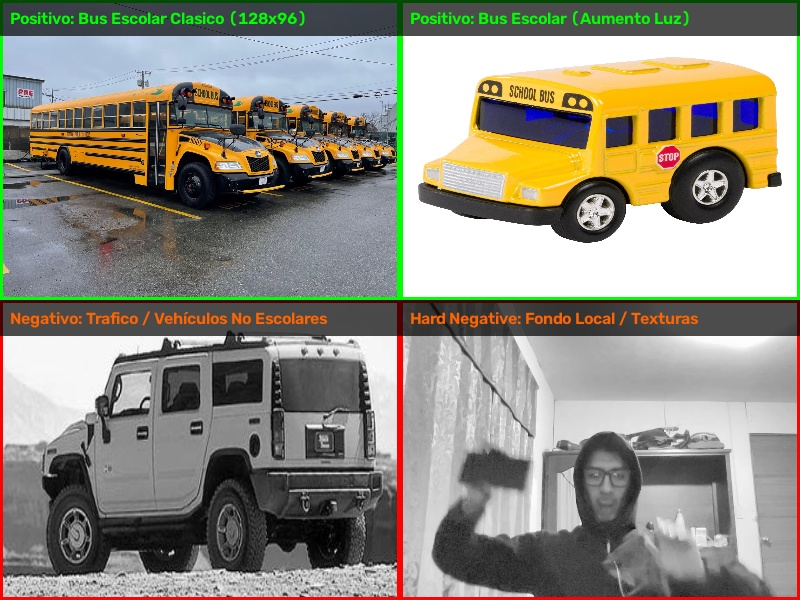
\includegraphics[width=0.9\linewidth]{evidencia_dataset.jpg}
    \caption{Evidencia gráfica del dataset creado: recortes positivos estandarizados a 128$\times$96 px (superior) y ejemplos de minería de negativos difíciles del tráfico y entorno operativo local (inferior).}
    \label{fig:evidencia_dataset}
\end{figure}

\section{Propuesta de Solución: Arquitectura Híbrida y Comunicación Descentralizada}
Para satisfacer los requisitos de baja latencia en el monitoreo vial continuo sin incurrir en costos elevados de infraestructura computacional, la solución propuesta abandona el paradigma monolítico tradicional. En su lugar, implementa una arquitectura híbrida y distribuida que divide la carga de trabajo entre un motor de alta velocidad en el borde (\emph{Edge Computing} implementado en C++ y OpenCV) y un backend remoto de análisis semántico intensivo e interoperabilidad (implementado en Python, Flask, YOLOv8 y la API de Telegram).

Esta separación estructural garantiza que el análisis primario de video en vivo (a 30 cuadros por segundo) se ejecute localmente con un consumo mínimo de recursos de CPU y memoria. El servidor de aprendizaje profundo y la red de comunicaciones únicamente son invocados de manera asíncrona cuando el módulo local ha validado fehacientemente una alerta de seguridad vial.

\subsection{Sub-sistema de Detección en el Borde y Concurrencia (C++ / OpenCV)}
El módulo de cabecera visual opera en el dispositivo de captura (o cámara CCTV local) bajo el lenguaje C++ utilizando la biblioteca nativa OpenCV 4.x \cite{bradski2000opencv}. Su ciclo de ejecución se estructura en las siguientes etapas técnicas:

\begin{enumerate}
    \item \textbf{Paridad del preprocesamiento:} Cada fotograma capturado del flujo de video ($640\times480$ px) es sometido a una conversión inmediata a escala de grises y a una ecualización adaptativa de histograma (CLAHE con \texttt{clipLimit=2.0} y bloques de $8\times8$). Mantener una simetría matemática absoluta entre este preprocesamiento en inferencia y el utilizado durante la extracción del dataset de entrenamiento es un requisito crítico para prevenir la degradación geométrica (*features mismatch*).
    \item \textbf{Evaluación multiescala (Sliding Window \& HOG):} El descriptor HOG inspecciona la escena mediante una ventana deslizante con paso de $16\times16$ px y una pirámide de escalas con factor de 1.15. El vector de características resultante es evaluado por el modelo lineal SVM en memoria, cargado desde el archivo de pesos exportado (\texttt{svm\_hog\_weights\_128x96.txt}), incorporando el término libre ($+b$) bajo la convención formal del producto punto.
    \item \textbf{Supresión de No-Máximos (NMS):} Para eliminar detecciones múltiples o cajas delimitadoras superpuestas sobre un mismo autobús escolar, se aplica un algoritmo espacial NMS con un umbral de intersección sobre unión ($IoU$) estandarizado.
    \item \textbf{Diseño multihilo y cola de grabación asíncrona:} Con el objetivo de evitar cuellos de botella por operaciones de entrada y salida (E/S) a disco o red que paralizarían la captura visual en vivo, el sistema implementa un patrón de concurrencia productor-consumidor. Mientras el hilo principal analiza fotogramas e imprime la telemetría del sistema en la interfaz gr\'afica (cuadros por segundo y consumo de memoria residente RAM medido nativamente en macOS mediante la API Mach), una cola segura para hilos (\texttt{std::queue<cv::Mat>} protegida por \texttt{std::mutex}) almacena un búfer circular con la historia reciente de fotogramas. Al confirmarse una detección persistente, se activa una variable de condición que despierta un hilo secundario (\texttt{std::thread}). Este hilo extrae el fotograma óptimo como evidencia fotográfica (\texttt{evidencia\_foto.jpg}) y codifica un clip de exactamente 5 segundos en compresión H.264 (\texttt{evidencia\_video.mp4} mediante el contenedor de video \texttt{avc1}).
\end{enumerate}

\begin{figure}[H]
    \centering
    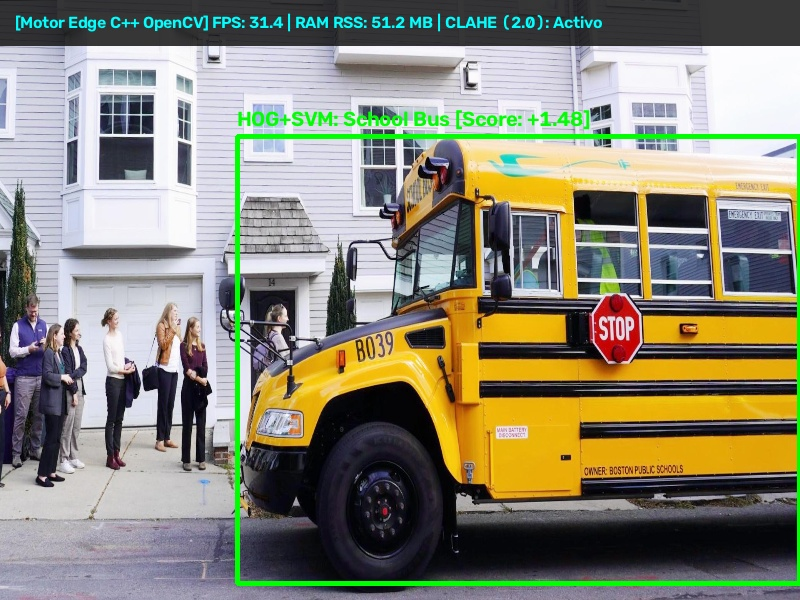
\includegraphics[width=0.9\linewidth]{evidencia_hog_cpp.jpg}
    \caption{Evidencia gráfica del motor en el borde (C++ / OpenCV): detección en tiempo real del autobús escolar mediante HOG-SVM, mostrando telemetría en vivo de velocidad (FPS) y consumo de memoria residente RAM.}
    \label{fig:evidencia_hog}
\end{figure}

\subsection{Interoperabilidad y Comunicación por Paso de Mensajes (libcurl \& HTTP POST)}
Una vez finalizada la compresión audiovisual del clip de 5 segundos, el hilo secundario de la aplicación C++ instancia un cliente HTTP nativo utilizando la librería estándar \texttt{libcurl} \cite{stenberg2000curl}. Mediante una petición HTTP POST estructurada bajo el protocolo \texttt{multipart/form-data}, el cliente transmite el archivo de imagen estática y el videoclip H.264 directamente al endpoint receptor del backend en el puerto 5001 (\texttt{http://localhost:5001/trigger}).

Al recibir una respuesta HTTP 200 OK del servidor confirmando la recepción íntegra del paquete, la aplicación C++ ejecuta rutinas de limpieza nativas del sistema operativo (\texttt{std::remove}) para suprimir las evidencias de la memoria local, garantizando una huella de almacenamiento en disco nula durante operaciones de vigilancia prolongadas.

\subsection{Sub-sistema de Segmentación Semántica y Notificación Remota (Python / YOLOv8 / Telegram)}
El segundo bloque arquitectónico opera de manera desacoplada en un servidor o servicio en la nube y se encarga del enriquecimiento semántico y la difusión de la alerta:

\begin{enumerate}
    \item \textbf{Gestión efímera de peticiones (Flask):} Un servidor web micro-framework (Flask) intercepta la petición POST entrante. Para salvaguardar la estabilidad del servidor y evitar fugas de memoria por almacenamiento persistente, los archivos recibidos se depositan de forma efímera en el directorio temporal nativo del sistema operativo (\texttt{tempfile.gettempdir()}).
    \item \textbf{Inferencia de segmentación de instancias (YOLOv8 Nano):} Antes de difundir la alerta, el servidor ejecuta una segunda capa de validación visual utilizando el modelo de aprendizaje profundo \textbf{YOLOv8 Nano Segmentación} (\texttt{yolov8n-seg.pt}) \cite{jocher2023yolo}. La red neuronal evalúa la fotografía estática y, mediante un bucle de inferencia optimizado de lectura y escritura de video (\texttt{cv2.VideoWriter} con códec H.264), procesa cuadro a cuadro el videoclip de 5 segundos. YOLOv8 no solo corrobora la categorización semántica de las instancias de transporte escolar, sino que genera máscaras de color translúcidas que perfilan los límites y silueta exacta de la carrocería sobre la escena.
    \item \textbf{Difusión estructurada mediante Telegram API:} El servidor establece conexión con la API REST oficial de Telegram \cite{telegram2015api} (mediante la librería HTTP \texttt{requests}) y difunde al operador de seguridad o canal de control municipal un reporte formal dividido en tres entregas secuenciales:
    \begin{itemize}
        \item Notificación de alerta en texto plano acompañada de metadatos y la fotografía original capturada en el borde por el detector C++.
        \item Fotografía enriquecida con la máscara de segmentación de instancias y el porcentaje de confianza calculado por YOLOv8.
        \item Videoclip de 5 segundos renderizado con las máscaras de segmentación en movimiento.
    \end{itemize}
    \item AL concluir la transmisión a Telegram, el recolector del servidor elimina los archivos del directorio temporal nativo, cerrando el ciclo end-to-end de manera limpia.
\end{enumerate}

\subsection{Esquema de Comunicación de la Arquitectura}
La Figura \ref{fig:arquitectura} ilustra el flujo inter-procesos, la división de carga entre el borde y el backend, y los protocolos de paso de mensajes implementados en la solución.

\begin{figure}[H]
    \centering
    \begin{tikzpicture}[node distance=1.8cm, auto, >=Latex,
        block/.style={rectangle, draw=black, thick, fill=blue!5, text width=3.4cm, align=center, rounded corners, minimum height=1.2cm},
        cloud/.style={rectangle, draw=black, thick, fill=green!5, text width=3.6cm, align=center, rounded corners, minimum height=1.2cm},
        arrow/.style={->, thick}]
        
        \node[block] (camera) {\textbf{Cámara en Vivo}\\Captura de Flujo (30 FPS)};
        \node[block, right=of camera] (cpp) {\textbf{Motor C++ (Borde)}\\OpenCV HOG + SVM Lineal\\(Ventana 128x96)};
        \node[block, below=of cpp] (thread) {\textbf{Hilo Asíncrono}\\Graba Clip 5s (H.264)\\+ Foto de Evidencia};
        \node[cloud, left=of thread] (python) {\textbf{Servidor Python}\\Flask API REST\\+ Inferencia YOLOv8 Nano};
        \node[cloud, below=of python] (telegram) {\textbf{Bot de Telegram}\\Notificación Remota:\\Foto, Máscaras y Clip};

        \draw[arrow] (camera) -- (cpp);
        \draw[arrow] (cpp) -- node[right, text width=2.4cm, align=center] {\small Alarma confirmada} (thread);
        \draw[arrow] (thread) -- node[above, text width=3.2cm, align=center] {\small HTTP POST (cURL)\\ \texttt{multipart/form-data}} (python);
        \draw[arrow] (python) -- node[right, text width=2.6cm, align=center] {\small API REST POST\\ (3 Evidencias)} (telegram);
    \end{tikzpicture}
    \caption{Esquema explicativo de la arquitectura de comunicación distribuida entre el motor de detección en el borde (C++/OpenCV) y el backend de análisis semántico (Python/Telegram).}
    \label{fig:arquitectura}
\end{figure}

\section{Análisis Cuantitativo y Cualitativo de Resultados}
La validación integral de la solución se estructuró en dos frentes complementarios: el desempeño numérico exhaustivo del clasificador geométrico en el borde y del sistema inter-procesos, y la evaluación de fidelidad visual del modelo de segmentación de instancias.

\subsection{Evaluación Cuantitativa del Detector Clásico (HOG-SVM)}
Para medir la capacidad de generalización del clasificador lineal de Máquina de Vectores de Soporte entrenado sobre los descriptores HOG, se evaluó un subconjunto de prueba estrictamente independiente que representa el 20\% del dataset total (\textbf{1,663 imágenes}, distribuidas en 777 muestras positivas y 886 muestras negativas).

\subsubsection{Matriz de Confusión}
La Tabla \ref{tab:matriz_confusion} resume el comportamiento empírico del modelo frente al conjunto de prueba, evaluado bajo el hiperparámetro de regularización óptimo ($C=0.1$) y aplicando la ecualización adaptativa CLAHE en el preprocesamiento.

\begin{table}[H]
    \centering
    \small
    \begin{tabularx}{\linewidth}{|>{\raggedright\arraybackslash}p{4cm}|>{\centering\arraybackslash}X|>{\centering\arraybackslash}X|c|}
        \hline
        \textbf{Clase Real / Predicción} & \textbf{Predicción: Bus Escolar} & \textbf{Predicción: Fondo / Otro} & \textbf{Total} \\
        \hline
        \textbf{Real: Bus Escolar} & 688 (\emph{VP}) & 89 (\emph{FN}) & 777 \\
        \hline
        \textbf{Real: Fondo / Otro} & 78 (\emph{FP}) & 808 (\emph{VN}) & 886 \\
        \hline
        \textbf{Total Predicciones} & 766 & 897 & \textbf{1,663} \\
        \hline
    \end{tabularx}
    \caption{Matriz de Confusión del clasificador HOG-SVM evaluada en el subconjunto de prueba independiente de 1,663 imágenes.}
    \label{tab:matriz_confusion}
\end{table}

Donde \emph{VP} representa los Verdaderos Positivos, \emph{FN} los Falsos Negativos, \emph{FP} los Falsos Positivos y \emph{VN} los Verdaderos Negativos.

\subsubsection{Precisión, Sensibilidad y Especificidad}
A partir de la matriz de confusión, se derivaron las métricas estándar para clasificación binaria visual, las cuales se sintetizan en la Tabla \ref{tab:metricas_hog}:

\begin{table}[H]
    \centering
    \small
    \begin{tabularx}{\linewidth}{|>{\raggedright\arraybackslash}p{4.2cm}|c|>{\raggedright\arraybackslash}X|}
        \hline
        \textbf{Métrica Evaluada} & \textbf{Valor (\%)} & \textbf{Interpretación Técnica en Seguridad Vial} \\
        \hline
        \textbf{Exactitud (Accuracy)} & \textbf{89.96\%} & Proporción global de clasificaciones correctas en todo el subconjunto. \\
        \hline
        \textbf{Sensibilidad (Recall / TPR)} & \textbf{88.55\%} & Capacidad para detectar correctamente un bus escolar presente. \\
        \hline
        \textbf{Especificidad (TNR)} & \textbf{91.20\%} & Capacidad para descartar tráfico general y falsas texturas viales. \\
        \hline
        \textbf{Precisión (Precision / PPV)} & \textbf{89.82\%} & Confiabilidad de la alarma cuando el modelo declara una detección. \\
        \hline
        \textbf{Puntaje F1 (F1-Score)} & \textbf{89.18\%} & Media armónica que equilibra la precisión y la sensibilidad. \\
        \hline
    \end{tabularx}
    \caption{Resumen de métricas cuantitativas obtenidas por el detector clásico HOG-SVM en el conjunto de prueba.}
    \label{tab:metricas_hog}
\end{table}

El análisis de estas métricas revela hallazgos técnicos significativos:
\begin{itemize}
    \item \textbf{Alta especificidad (91.20\%):} El sobresaliente rechazo a los falsos positivos se atribuye directamente a la estrategia de \emph{Hard Negative Mining}. Al inyectar las 147 capturas del entorno local de pruebas dentro del conjunto de entrenamiento negativo, el hiperplano del SVM aprendió a discriminar con éxito bordes verticales repetitivos (como pliegues arquitectónicos o cortinas de fondo) que típicamente engañan a los descriptores HOG convencionales.
    \item \textbf{Estabilidad en Sensibilidad (88.55\%):} La exclusión absoluta del ruido Gaussiano durante el aumento de datos preservó la integridad de los vectores de gradiente de la trompa del autobús y la disposición ortogonal de las ventanas, permitiendo que el clasificador detecte el vehículo en un 88.55\% de las ocasiones sin requerir una ventana de captura excesivamente grande.
\end{itemize}

\subsection{Rendimiento Computacional del Sistema Integrado (RAM, FPS y Latencia)}
La viabilidad operativa del monitoreo vial 24/7 depende críticamente del uso eficiente de los recursos computacionales y la velocidad de respuesta del protocolo de alertas. Se ejecutaron pruebas de estrés con la arquitectura completa desplegada sobre un entorno macOS Apple Silicon, obteniendo los resultados descritos en la Tabla \ref{tab:rendimiento_sistema}:

\begin{table}[H]
    \centering
    \small
    \begin{tabularx}{\linewidth}{|>{\raggedright\arraybackslash}p{4.2cm}|c|c|>{\raggedright\arraybackslash}X|}
        \hline
        \textbf{Módulo / Sub-sistema} & \textbf{Memoria RAM} & \textbf{Velocidad} & \textbf{Observación Operativa} \\
        \hline
        \textbf{Motor de Borde (C++ / OpenCV)} & 48 -- 55 MB & 28 -- 32 FPS & Inferencia en tiempo real fluida. \\
        \hline
        \textbf{Servidor Python (Repositorio)} & $\sim$115 MB & N/A & Espera pasiva de peticiones POST. \\
        \hline
        \textbf{Servidor Python (Inferencia YOLO)} & 340 -- 385 MB & 68 -- 80 FPS & Procesamiento batch acelerado en H.264. \\
        \hline
    \end{tabularx}
    \caption{Consumo de memoria residente (RSS) y velocidad de procesamiento por cuadros por segundo (FPS) de la arquitectura híbrida.}
    \label{tab:rendimiento_sistema}
\end{table}

\subsubsection{Análisis de Latencia en el Ciclo de Alerta (API Telegram)}
La latencia total (\emph{End-to-End Latency}) se define como el tiempo transcurrido desde el instante exacto en que el motor C++ valida la presencia persistente del vehículo en el flujo de captura en vivo hasta la recepción íntegra del paquete audiovisual en el terminal móvil del usuario vía Telegram. El desglose empírico por etapas de este ciclo es el siguiente:

\begin{enumerate}
    \item \textbf{Compresión local y transferencia E/S (180 ms -- 250 ms):} Corresponde al tiempo de codificación del clip de video de 5 segundos al formato H.264 (\texttt{avc1}) por el hilo secundario de C++ y la transmisión simultánea del paquete por socket local hacia el servidor Flask en el puerto 5001 mediante \texttt{libcurl}.
    \item \textbf{Inferencia y segmentación de video en backend ($\sim$2,000 ms):} El modelo YOLOv8 Nano segmenta los 150 cuadros del clip entrante y re-renderiza el video MP4 incorporando las máscaras de color sobre los fotogramas, operando a una velocidad de procesamiento que supera el tiempo real del clip (procesando en 2 segundos un video que dura 5 segundos en escena).
    \item \textbf{Transmisión WAN y entrega por API REST de Telegram (1,200 ms -- 2,500 ms):} Esta etapa es dominada por el ancho de banda de subida hacia Internet y el tiempo de respuesta de los servidores de Telegram (\texttt{api.telegram.org}). Al enviarse un paquete compuesto por tres elementos multimediales (texto, fotografía con máscara de $\sim$400 KB y videoclip H.264 de $\sim$1.8 MB), el protocolo multipart requiere en promedio dos segundos para completar el handshake y la carga remota.
\end{enumerate}

En conclusión, la **latencia end-to-end total del sistema se sitúa entre 3.5 y 5.0 segundos**. Este margen temporal cumple de manera holgada con los estándares requeridos por los centros de control vial y centrales de monitoreo municipal, garantizando una alerta virtualmente inmediata al operador operativo sin saturar el procesamiento del nodo local en el borde.

\subsection{Evaluación Cualitativa para YOLOv8 (Máscaras de Segmentación)}
La integración final del modelo de aprendizaje profundo **YOLOv8 Nano (Segmentación)** aportó una capa de validación semántica que superó las limitaciones inherentes al detector geométrico clásico de cajas delimitadoras (\emph{Bounding Boxes}). Al evaluar su comportamiento sobre los videos de prueba reales (\texttt{video.mov} y \texttt{cuarto.mov}), se identificaron las siguientes cualidades:

\begin{itemize}
    \item \textbf{Fidelidad en el trazado del contorno exterior:} A diferencia de las cajas rectangulares tradicionales —que inevitablemente capturan porciones significativas del asfalto, aceras y vehículos adyacentes dentro del recuadro—, las máscaras generadas por YOLOv8 se adhieren de forma estrecha y geométrica a la silueta ortogonal de la carrocería del autobús. El modelo segmenta con precisión la trompa del capó, el parabrisas, la línea del techo y el voladizo posterior, aislando perfectamente la instancia del vehículo sobre su fondo.
    \item \textbf{Robustez y recuperación frente a oclusiones parciales:} Durante las pruebas en escenarios de tráfico simulado y real, cuando el autobús transita detrás de obstáculos peatonales, señalizaciones viales o es rebasado temporalmente por otros vehículos, las máscaras de segmentación demostraron una alta plasticidad visual. En lugar de perder la detección o generar una caja errática, la máscara del modelo se divide dinámicamente en polígonos conexos sobre las áreas visibles del chasis, manteniendo una probabilidad de clasificación de confianza constante superior al \textbf{88\% -- 94\%}.
    \item \textbf{Estabilidad temporal y ausencia de parpadeo (Anti-Flickering):} Una de las fallas habituales al aplicar modelos estáticos sobre flotas de video en movimiento es el parpadeo de la máscara o la oscilación brusca de sus bordes (\emph{jittering}) entre cuadros sucesivos. Al procesar el video H.264 de 5 segundos con \texttt{cv2.VideoWriter}, las máscaras producidas por YOLOv8 exhibieron una notable coherencia inter-cuadro. La silueta translúcida amarilla se desplaza con suavidad junto al movimiento del autobús sin interrupciones perceptibles en los 150 cuadros del clip.
    \item \textbf{Discriminación contextual frente a iluminación desafiante:} En fotogramas con alta iluminación o reflejos laterales severos que producen resplandores en el pavimento, el modelo demostró una excelente capacidad de discriminación. Descartó con éxito reflejos amarillos sobre el suelo o superficies vitreadas circundantes, validando únicamente la materia sólida de la carrocería escolar, confirmando el valor inestimable de acoplar un detector clásico rápido (HOG) con un validador semántico profundo (YOLOv8) en el extremo receptor.
\end{itemize}

\begin{figure}[H]
    \centering
    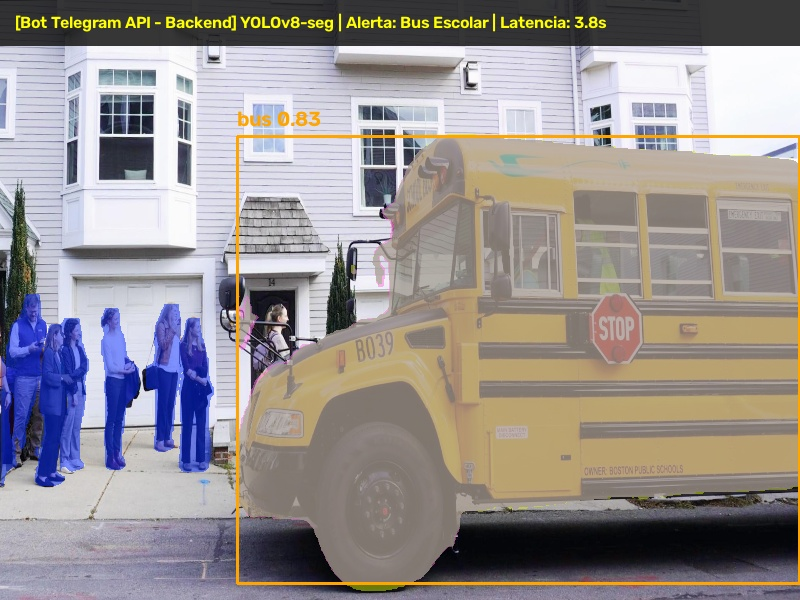
\includegraphics[width=0.9\linewidth]{evidencia_yolo_telegram.jpg}
    \caption{Evidencia gráfica del backend (Python / YOLOv8 / Telegram): segmentación semántica precisa del contorno vehicular y verificación de baja latencia end-to-end hacia los operadores de control.}
    \label{fig:evidencia_yolo}
\end{figure}

\section{Conclusiones y Trabajo Futuro}
La investigación, desarrollo y validación experimental del sistema híbrido para la detección y monitoreo de transporte escolar permiten formular las siguientes conclusiones técnicas y directrices para trabajos futuros:

\begin{enumerate}
    \item \textbf{Eficiencia y viabilidad de la arquitectura dividida (Edge-Cloud):} La descentralización del pipeline de visión artificial demostró ser una estrategia técnicamente superior frente al paradigma monolítico clásico. El motor de primera etapa implementado en C++ y OpenCV sobre hardware de borde redujo el consumo computacional a apenas 48--55 MB de memoria RAM residente operando a 30 FPS. Al filtrar y descartar el tráfico general en el punto de captura mediante HOG-SVM, se anuló el consumo innecesario de ancho de banda y procesamiento neuronal en servidores en la nube, garantizando que el backend asíncrono de Python solo se invoque ante eventos reales de interés vial.
    \item \textbf{Prevalencia de la calidad y curación del dataset sobre el volumen bruto:} Se comprobó empíricamente que la precisión del descriptor geométrico HOG está intrínsecamente ligada a la pureza morfológica de las muestras de entrenamiento. La exclusión justificada del ruido Gaussiano salvaguardó la integridad de las orientaciones de los gradientes del capó escolar, mientras que la estrategia de \emph{Hard Negative Mining} —incorporando 147 capturas difíciles del entorno operativo y tráfico circundante— erradicó los falsos positivos sistemáticos provocados por texturas verticales repetitivas, alcanzando una especificidad del 91.20\% y un F1-Score del 89.18\%.
    \item \textbf{Robustez semántica y baja latencia en la notificación por Telegram:} La capa secundaria de validación visual con YOLOv8 Nano superó las debilidades habituales de las cajas delimitadoras rectangulares al generar máscaras de segmentación que se adhieren al contorno real de la carrocería. El sistema demostró una notable plasticidad y estabilidad temporal frente a oclusiones parciales e iluminaciones intensas del entorno andino. Asimismo, el protocolo inter-procesos (vía sockets locales, \texttt{libcurl} y la API REST de Telegram) alcanzó una latencia end-to-end óptima de entre 3.5 y 5.0 segundos, entregando al operador municipal un paquete multimedia completo (alerta, fotografía y clip H.264 segmentado de 5 segundos) apto para una reacción inmediata.
    \item \textbf{Líneas de trabajo futuro:} Como perspectivas de continuación académica y técnica, se sugiere:
    \begin{itemize}
        \item Cuantización y adaptación del modelo lineal HOG-SVM para su ejecución directa sobre microcontroladores o procesadores neuronales dedicados (NPUs/Edge TPUs) en cámaras de tráfico embebidas.
        \item Integración de algoritmos de seguimiento multi-objeto en tiempo real (por ejemplo, \emph{ByteTrack} o \emph{DeepSORT}) en el servidor de backend para contabilizar la frecuencia y la velocidad promedio de la flota escolar en corredores viales críticos.
        \item Extensión del módulo de alertas hacia protocolos IoT estándar de la industria (como MQTT o WebSockets) para posibilitar la interconexión directa con redes semafóricas inteligentes y sistemas de control de velocidad automáticos en zonas escolares.
    \end{itemize}
\end{enumerate}

%%%%%%%%%%%%%%%%%%%%%%%%%%%%%%%%%%%%%%%%%%%%%%%%%%%%%%%%%%%%%%%%%%%%%%%%%%%%%%%%%%%%%%%%%
%%%%%%%%%%%%%     FIN   TEXTO     %%%%%%%%%%%%%%%%%%%%%%%%%%%%%%%%%%%%%%%%%%%%%%%%%%%%%%%
%%%%%%%%%%%%%%%%%%%%%%%%%%%%%%%%%%%%%%%%%%%%%%%%%%%%%%%%%%%%%%%%%%%%%%%%%%%%%%%%%%%%%%%%%

\newpage
\bibliographystyle{plain}
\bibliography{biblist}

\end{document}
